%%%%%%%%%%%%%%%%%%%%%%%%%%%%%%%%%%%%%%%%%
% baposter Portrait Poster
% LaTeX Template
% Version 1.0 (15/5/13)
%
% Created by:
% Brian Amberg (baposter@brian-amberg.de)
%
% This template has been downloaded from:
% http://www.LaTeXTemplates.com
%
% License:
% CC BY-NC-SA 3.0 (http://creativecommons.org/licenses/by-nc-sa/3.0/)
%
%%%%%%%%%%%%%%%%%%%%%%%%%%%%%%%%%%%%%%%%%

%----------------------------------------------------------------------------------------
%	PACKAGES AND OTHER DOCUMENT CONFIGURATIONS
%----------------------------------------------------------------------------------------

\documentclass[a0paper,portrait]{baposter}

\usepackage[font=small,labelfont=bf]{caption} % Required for specifying captions to tables and figures
\usepackage{booktabs} % Horizontal rules in tables
\usepackage{relsize} % Used for making text smaller in some places
%\usepackage{palatino}
\usepackage{helvet}
\renewcommand{\familydefault}{\sfdefault}
\usepackage[sort]{natbib}%square,
\usepackage{amsmath, amssymb}
\usepackage{enumitem}

\graphicspath{{/}} % Directory in which figures are stored #figures/

\definecolor{bordercol}{RGB}{40,40,40} % Border color of content boxes
\definecolor{headercol1}{RGB}{186,215,230} % Background color for the header in the content boxes (left side)
\definecolor{headercol2}{RGB}{80,80,80} % Background color for the header in the content boxes (right side)
\definecolor{headerfontcol}{RGB}{0,0,0} % Text color for the header text in the content boxes
\definecolor{boxcolor}{RGB}{186,215,230} % Background color for the content in the content boxes

\definecolor{udsect}{rgb}{0.184,0.31,0.31} 
\definecolor{wurblue}{rgb}{0,0.298,0.471}

\begin{document}

%\background{ % Set the background to an image (background.pdf)
%\begin{tikzpicture}[remember picture,overlay]
%\draw (current page.north west)+(-2em,2em) node[anchor=north west]
%{\includegraphics[height=1.1\textheight]{background}};
%\end{tikzpicture}
%}

\begin{poster}{
grid = false,
borderColor=bordercol, % Border color of content boxes
headerColorOne=white, % Background color for the header in the content boxes (left side)
headerColorTwo=white, % Background color for the header in the content boxes (right side)
headerFontColor=black, % Text color for the header text in the content boxes
boxColorOne=white, % Background color for the content in the content boxes
headershape=smallrounded, %roundedright, % Specify the rounded corner in the content box headers
headerfont=\Large\sf\bf, % Font modifiers for the text in the content box headers
textborder=roundedsmall,
background=shadeLR, %user
headerborder=open, % Change to closed for a line under the content box headers
boxshade=plain , %,
bgColorOne=udsect,
bgColorTwo=udsect
}
{}
%
%----------------------------------------------------------------------------------------
%	TITLE AND AUTHOR NAME
%----------------------------------------------------------------------------------------
%
{\sf \bf \huge \textcolor{white}{\textsc{Quantifying LD decay by quantile regression \\[0.25em] a case study }}} % Poster title
{\vspace{0.8em}  \textcolor{white}{\textsc{Sabine K.Schnabel$^{1}$, Federico Torretta$^{2}$ and Matthias Westhues$^{3}$}}\\ % Author names
{\small \textcolor{white}{1: Biometris, Wageningen University and Research Centre, The Netherlands; 
2: Universit\`a di Palermo, Italy; 3: Universit\"at Hohenheim, Germany }}} % Author email addresses
%{\includegraphics[scale=0.25]{log-pdf-wu-emc}
%} % University/lab logo


%----------------------------------------------------------------------------------------
%	INTRODUCTION
%----------------------------------------------------------------------------------------

%\headerbox{\textsc{Introduction}}{name=introduction,column=0,row=0}{

\headerbox{\textsc{Introduction}}{name=introduction,span=3, column=0, row=0}{
\vspace{-0.5cm}
\begin{minipage}{0.3 \textwidth}
\begin{itemize}[leftmargin=*]
	\item Genome-wide association studies: great tool for the 
	localization of QTLs (quantitative trait loci) in plant and animal breeding programs.
	\item Investigation of the genetic relatedness (kinship matrix) required for powerful GWAS %\citep{astle2009} 
		\begin{itemize}[leftmargin=*]
		\item[$\rightarrow$] Insight into LD between genetic markers necessary %\citep{Listgarten2012}
		\end{itemize}
\end{itemize}  
%For an appropriate kinship matrix, insight into LD between 
%genetic markers is necessary.  propose to base this matrix on a set of independent markers.

%Expectiles have become popular in the last years.
%		\begin{itemize}[leftmargin=1.5em]
%			\item[$\rightarrow$] But for big data calculations are computationally intensive.
%		\end{itemize}
%
%\textbf{Application from plant sciences:} visualization of relation of 
%		linkage disequilibrium (LD) decay 
%		  and the distance between SNPs
%\\[0.2cm]
%\textbf{Basic idea:} correlation between pairs of SNPs $\rightarrow$ millions of 
%pairs from thousands of markers
\end{minipage}
%
\hspace{0.4cm}
\begin{minipage}{0.33 \textwidth}
\vspace{0.5cm}
\centering
Global LD decay on Chromosome 1
\begin{center}
\vspace{-1.5cm}
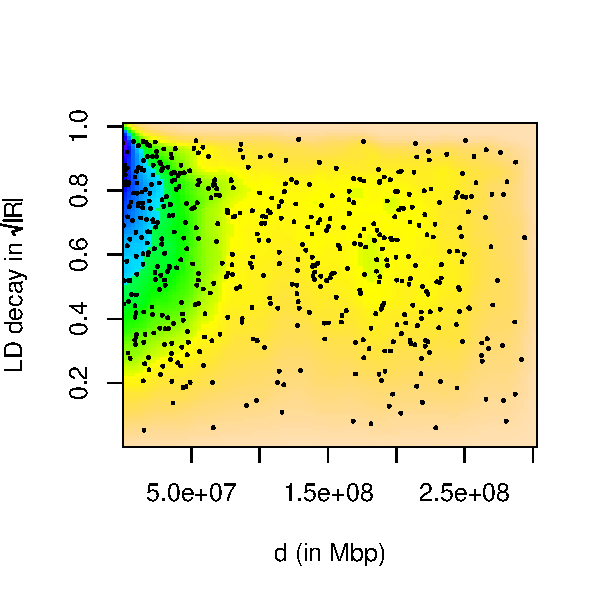
\includegraphics[width=0.8\linewidth]{SchnabelTorrettaWesthuesFigure1A}
\end{center}
\vspace{-0.2cm}
\end{minipage}
%
%\hfill
\hspace{0.6cm}
\begin{minipage}{0.3 \textwidth}
\begin{itemize}[leftmargin=*]
	\item Find suitable set of independent markers 
	\item Exploration of LD decay over the whole genome
	\item LD is commonly measured in terms of the squared Pearson correlation coefficient $R^2$ between pairs 
		of genetic markers \citep{Hill1968}. 
\end{itemize}
%To find such a set of suitable markers (e.g. single nucleotide polymorphism -- SNP) we need 
%to explore LD decay over the whole genome. LD is commonly measured in terms of 
%the squared Pearson correlation coefficient $R^2$ between pairs of genetic
%markers \citep{Hill1968}. 
%As an example, we are using data from chromosome 1 of a Maize 
%population consisting of 123 European Dent inbred lines and 114 European Flint inbred lines
%\citep{Fischer2008}. Figure~\ref{SchnabelTorrettaWesthues:fig1}(A) shows an LD decay plot 
%for this part of the genome.\\
%\vspace{-1.4cm}
%We are proposing the following approach:
%\begin{itemize}[leftmargin=*]
%\item Describe the steps
%%\item Summarize the data on a grid \newline $\rightarrow$ 2D histogram 
%%\item Estimate expectile curves using:
%%	\begin{itemize}[leftmargin=*]
%%		\item Fast matrix calculations
%%		\item Discrete smoother with weights	  
%%	\end{itemize}	
%\end{itemize}
\end{minipage}
}%

%----------------------------------------------------------------------------------------
%	MATERIALS AND METHODS
%----------------------------------------------------------------------------------------
\headerbox{\textsc{Quantile regression}}{name=QR,column=1,below=introduction} {%, bottomaligned=histogram}{
\begin{itemize}[leftmargin=*]
	\item Using non-parametric quantile 
	regression with a monotonicity constraint \citep{Muggeo2013,BollaertsEtAl2006StatMod}
	\item Monotone decreasing curve is in line with biological assumptions.
	\item $\mu_{\tau}=s_{\tau}(d)$, $\mu_\tau$ quantile function at 
	percentile $\tau$, $d$ SNP distance between pairs of markers and 
	$s_{\tau}(\cdot)$ smooth and unknown function
	\item  $P-$splines for a smooth functional form, therefore: \newline 
$\min\sum_k^K b_{k\tau} B_k(d)$ subject to $b_k<b_{k-1}$ for $k=2,\ldots,K$, with $b_{k\tau}$
	the coefficient of the $B_k$-th spline, $K$ the dimension of the design matrix.
	\newline $\mbox{}$
%\item 
%	If you want to add something more you could include one of the following:
%		\item \[w_{\tau,i} =\left\{
%		\begin{array}{lr}
%		\tau  &  y_i\geq \mu_i\\
%		1-\tau  &  y_i < \mu_i
%		\end{array}
%		\right.
%		\]
%		\item $\mathcal{R}(b_j; \tau)= 
%		\sum_{i=1}^n w_{\tau,i}|y_i-\sum_{j}^{J}b_jB_{j}(dist_i)| +\lambda \sum^{J-d}_{j=1}\left|D_d b\right|_j$
%	\end{itemize}
%		where $D_d$ is the $d$-order difference operator 
%		and $\lambda$ is the smoothing parameter
%	
%
\end{itemize}
}


\headerbox{\textsc{Data and Visualization}}{name=histogram,column=0, below=introduction, bottomaligned=QR}{
\begin{itemize}[leftmargin=*]
\item Data from Maize population \citep{Fischer2008}, especially from Chromosome 1 with almost 5000 markers $\rightarrow$ more than 12 million pairwise comparisons
\item For these large data: visualization is difficult in a scatterplot. 
\item Apply a scatterplot smoother \citep{Eilers22032004} 
	\begin{itemize}[leftmargin=*]
	\item[$\rightarrow$] computation of a
			two-dimensional histogram, smoothing of the counts and display with a color map
	\end{itemize}
\item In order to improve the quality of the fit and the visualization $\rightarrow$ use of $\sqrt{|R|}$ instead 
of Pearson's $R^2$.
\end{itemize}
%
%Chromosome 1 of the above described 
%Maize genome has almost 5000 markers, resulting in more than 
%12 million pairwise comparisons 
%	between two markers on the same chromosome. Visualization of these large data sets is 
%	challenging. We used a scatterplot smoother (Eilers and Goeman, 2004) for depicting
%	global LD decay on chromosome 1 (length $\approx$ 300 Mbp (Mega base pairs))   
%	in Figure~\ref{SchnabelTorrettaWesthues:fig1}(A). As mentioned above, the most 
%	common measure for LD decay is the squared Pearson correlation $R^2$. In order to improve the 
%	quality of the fit as well as the visualization, we advocate to use $\sqrt{|R|}$ instead. Further 
%	investigation concerning this transformation will be reported elsewhere. 
%\begin{itemize}[leftmargin=*]
%%	\item Summarizing the data on a grid of 100 $\times$ 100 bins reduces any size of data to $10^4$ 
%%		pseudo-observations.
%%	\item Use of midpoints and counts as weights	
%%%	\item The two-dimensional histogram can be constructed quickly in \texttt{R}.
%%%The simplest approach is to just run a loop over all
%%%observations. That takes 3 to 5 seconds for one million
%%%observations. Compilation to byte code ---using {\tt cmpfun} in
%%%the {\tt compiler} package--- reduces this time by a factor five. The
%%%fastest solution however is to apply the {\tt hist} function. 
%%%Let $j_i$ and $k_i$ be the row and column indices of
%%%observation~$i$. Let $h_i = j_i + n k_i$ be a combined index.
%%%The one-dimensional histogram of $h$ with $n^2$ bins can be
%%%re-dimensioned to the desired $n$-by-$n$ matrix. This speeds
%%%up the calculations by another five times.
%	\item For larger data sets: visualization is difficult in a scatterplot. 
%	\item Apply a scatterplot smoother \citep{Eilers22032004} 
%		\begin{itemize}[leftmargin=*]
%		\item[$\rightarrow$] computation of a
%				two-dimensional histogram, smoothing of the counts and display with a color map
%		\end{itemize}
%\end{itemize}
}




\headerbox{\textsc{Global/local LD}}{name=LD,column=2,below=introduction, bottomaligned=QR}{
%
%
%	In our case, it is of interest to examine what happens to 
%	LD decay on a smaller scale. Therefore we investigate local LD decay in subsequent 
%	overlapping sliding windows of 2.5 Mbp width and fit a set of quantile curves to each of these 
%	sections of the whole plot.  

\begin{itemize}[leftmargin=*]
\item Usually analysis focusses on the global LD decay (per chromosome) $\rightarrow$ general picture about the 
	linkage desequilibrium and linkage between the markers
\item Here: emphasis on local LD decay to get more insights on a smaller scale
	\begin{itemize}[leftmargin=*]
	\item Overlapping sliding windows of 2.5 Mbp $\rightarrow$ around 1000 windows on chromosome 1 with on average 
			2000 points per window
	\item Fit a set of quantile curves to each of the windows (here $\tau=0.25, 0.5, 075$)
	\item Choose threshold $T$ in terms of $R^2$ and collect the associated distances from whereon LD decay is 	
		lower than $T$
	\end{itemize}
%	\item Expectiles are an interesting and useful alternative to quantiles.
%	\item Fast and easy calculation using iteratively reweighted least squares 
%	\item Estimation using LAWS
%	\vspace{-0.2cm}
%		\begin{itemize}[leftmargin=*]
%			\item[] Minimize \newline
%  					$Q = (y - B\alpha)^T W_p(y - B\alpha) + \lambda ||D\alpha||^2$ \newline
%				   with diagonal weight matrix $W_p$ defined as:  
%				   %\vspace{-0.2cm}
%					$ \left\{\begin{array}{ll}
%							w_{ii} = p 	 &\mbox{ if $y_i > \hat y_i$};\\
%							w_{ii} = 1-p &\mbox{ otherwise.}	
%						\end{array}
%					\right.$
%			\item[] Solve repeatedly and update $W_p$: \newline
%  				$(B^T W_pB + \lambda D^T D) \alpha = B^T W_py$
%%is solved repeatedly, updating the elements of $W_p$  after
%%each iteration. This is the least asymmetrically weighted
%%squares (LAWS) algorithm. It converges quickly to the minimum
%%of $Q$, which is a convex function of $\alpha$. For visualization, one computes and
%%plots the curves for a set of values of $p$.
%
%		\end{itemize}				
%\item Computationally intensive for big data %large data sets
\end{itemize}
}







\headerbox{\textsc{Results}}{name=results,column=0, span=3 ,below=QR}{
\begin{minipage}{0.24\textwidth}
\vspace{-0.8cm}
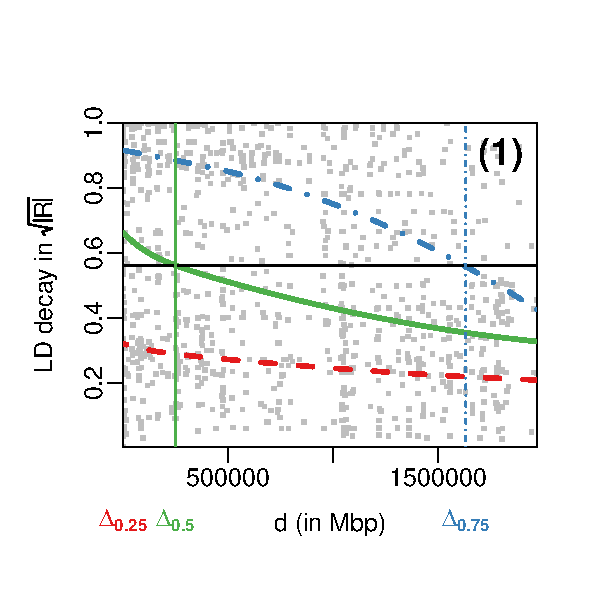
\includegraphics[width=0.95\linewidth]{SchnabelTorrettaWesthuesFigure1B}
\end{minipage}
%
\begin{minipage}{0.24 \textwidth}
Some text
\end{minipage}
%
%\hfill
\hspace{1.5cm}
\begin{minipage}{0.48\textwidth}
\vspace{-0.8cm}
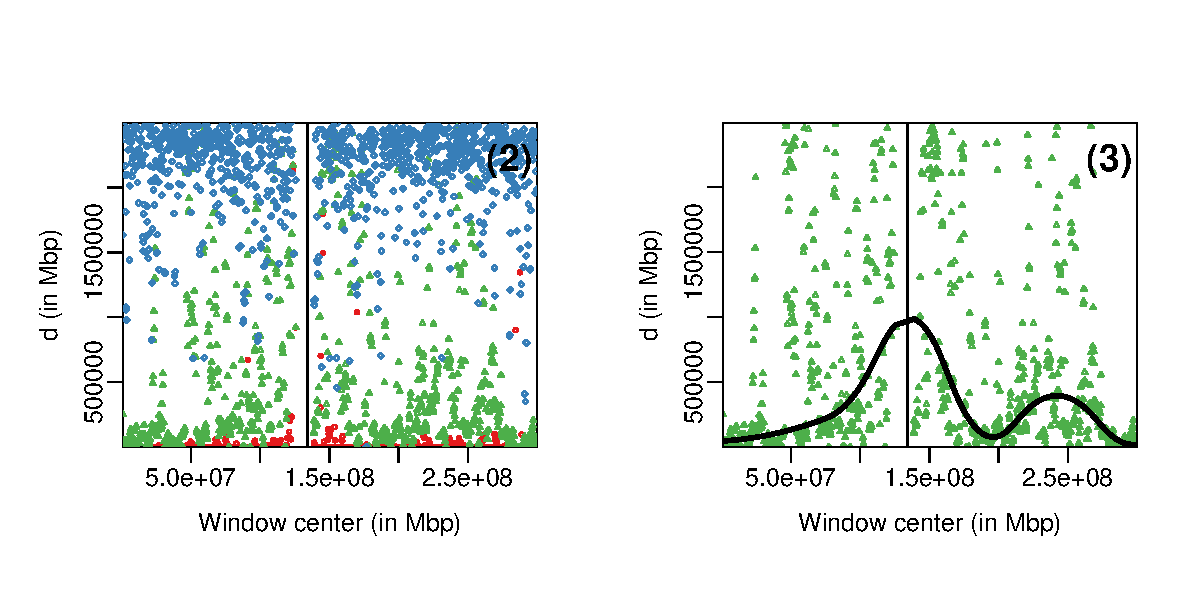
\includegraphics[width=0.95\linewidth]{SchnabelTorrettaWesthuesFigure1CD}
\end{minipage}
%\begin{minipage}{0.5\textwidth}
%\begin{center}
%\vspace{-0.6cm}
%\includegraphics[width=0.9\linewidth]{SchnabelFigure1_new_13042015_long}
%\vspace{-0.5cm}
%
%\end{center}
%\end{minipage}
%%
%\begin{minipage}{0.5\textwidth}
%\begin{center}
%\vspace{-0.6cm}
%\includegraphics[width=0.9\linewidth]{SchnabelFigure2_new_13042015_long}
%\vspace{-0.5cm}
%\end{center}
%\end{minipage}
}


\headerbox{\textsc{Conclusion and Discussion}}{name=beyond,column=0, span=3
 ,below=results}{
 \begin{minipage}{0.48\textwidth}
\begin{itemize}[leftmargin=*]
\item Case study of how to explore and quantify local LD decay patterns in Maize using
 quantile regression with monotonicity constraints for a first summary of the LD decay. 
\item  Applying $P-$splines to smooth the median local LD decay $\rightarrow$ 
	easy to interpret and inspect for the collaborating biologists 
\item In depth exploration of local LD decay (in comparison to global LD decay) leads to
		new insights.	
\end{itemize}
\end{minipage}
%
\hfill
\begin{minipage}{0.48\textwidth}
\begin{itemize}[leftmargin=*]
\item In addition to a good tool to quantify local LD decay $\rightarrow$ also an instrument in identifying 
	problems with the underlying genotypic 
 	data that have previously been 
 	overlooked. 
\item Can serve as a diagnostic tool
	\begin{itemize}[leftmargin=*]
	\item Discovering of undercoverage through sliding windows with low sample sizes
	\item Clustering of correlation values $\rightarrow$ unknown phenomenon in the data, adjustment in subsequent 
		analysis
	\end{itemize}
\end{itemize}	
 \end{minipage}
% 	\item Adapt the grid algorithm for quantile curves using \citep{Schlossmacher1973}: \newline
%		 $S= \sum_i |u_i| \rightarrow \tilde{S} = \sum_i u_i^2/|\tilde{u}_i|$, 
% 			see also \citep{SchnabelEilersQSPublished}
% 	\item Shape constraints \citep{Eilers2005UnimodalSmoothing}		
% %	\item Conditional densities \citep{STA4:STA427}
% 	\item Investigation of other shapes of the data cloud 
% 		%How to adapt the histogram/bin number/size when data comes in different shapes? 
% %	\item Test bundle and expectile sheets? Probably not necessary with the huge amount of data. No crossing to be 
% %			expected.
% 	\item Smoothing parameters \citep{SchnabelEilers}
% 	\item Transformation of the response to get more insight into the relationship
% \end{itemize}
}

%\headerbox{\textsc{Fit to transformed data}}{name=illustration,column=2, below=results, bottomaligned=beyond}{
%\begin{center}
%\vspace{-0.4cm}
%\includegraphics[width=0.95\linewidth]{SchnabelFigure5_mon_simu_sqrt_13042015_long}
%\end{center}
%}

\headerbox{\textsc{Acknowledgements}}{name=ack, column=0, span=2, below=beyond, above=bottom}{
%\vspace{-0.7cm}
\begin{minipage}{0.7\linewidth}
This case study was performed while FT and MW were 
visiting at Biometris at Wageningen University and Research Centre in Winter 2014/2015. We are indebted to the group of Prof. Dr. Ruedi Fries, from Technische Universit\"at M\"unchen, for the SNP genotyping of the parental lines, which was funded by the German Federal Ministry of Education and Research (BMBF)  within the AgroClustEr ''Synbreed-Synergistic plant and animal breeding'' (FKZ:0315528d).
\end{minipage}
%
%\hfill
\hspace{0.1cm}
\begin{minipage}{0.25\linewidth}
%\hspace{0.5em}
%\vspace{-0.4cm}
\centering
%\includegraphics[scale=0.25]{log-pdf-wu-emc}
\includegraphics[scale=0.40]{wu}
\vspace{-0.2cm}
\includegraphics[scale=0.19]{logoUNIPA}
\includegraphics[scale=0.23]{Uni_Hohenheim_Logo_blau_GB}
\end{minipage}
}%

\headerbox{\textsc{References}}{name=Ref,span=1, column=2,below=beyond, above=bottom}{
%\begin{minipage}{0.41\textwidth}
%\vspace{-0.0cm}
\renewcommand{\section}[2]{\vskip 0.05em} % Get rid of the default "References" section title
\tiny%\scriptsize
\bibliographystyle{genetics}
\vspace{-0.1cm}
\bibliography{litIWSM2015_poster}
%\end{minipage}
}


%\headerbox{\textsc{References}}{name=acknowledgementsRef,span=3, column=0,below=beyond, above=bottom}{
%
%\begin{minipage}{0.28\linewidth}
%%\hspace{0.5em}
%\vspace{-0.6cm}
%\centering
%%\includegraphics[scale=0.25]{log-pdf-wu-emc}
%\includegraphics[scale=0.45]{wu}
%\includegraphics[scale=0.2]{logoUNIPA}
%\includegraphics[scale=0.25]{Uni_Hohenheim_Logo_blau_GB}
%
%\end{minipage}
%%
%\begin{minipage}{0.72\linewidth}
%\renewcommand{\section}[2]{\vskip 0.05em} % Get rid of the default "References" section title
%\scriptsize
%\bibliographystyle{genetics}
%\vspace{-0.1cm}
%\bibliography{IWSM2014Bib} %{litIWSM2015_poster}
%\end{minipage}
%
%}

%\headerbox{\textsc{}}{name=acknowledgements,column=0,below=beyond, above=bottom}{
%\hspace{0.5em}
%\includegraphics[scale=0.25]{log-pdf-wu-emc}
%} 
%
%\headerbox{\textsc{References}}{name=references,span=2,column=1,below=beyond,above=bottom}{ % To reduce this block to 1 column width, remove 'span=2'
%
%%\smaller % Reduce the font size in this block
%\renewcommand{\section}[2]{\vskip 0.05em} % Get rid of the default "References" section title
%%\nocite{*} % Insert publications even if they are not cited in the poster
%\scriptsize
%\bibliographystyle{genetics}
%%\def\newblock{}
%\bibliography{IWSM2014Bib}
%
%%\bibliographystyle{unsrt}
%%\bibliography{sample} % Use sample.bib as the bibliography file
%}



%----------------------------------------------------------------------------------------

\end{poster}

\end{document}


%\documentclass[a4paper,10pt]{report}
%\usepackage[utf8]{inputenc}
%
%\title{Formula for Sabine}
%\begin{document}
%\maketitle
%
%This is the formula that we excluded afterwards:
%
%$\min\sum_k^K b_{k\tau} B_k(dist)$ subject to $b_k>b_{k-1}$ for $k=2,\dots,K$, \\
%
%	where $b_{k\tau}$
%	is the coefficient of the $B_k$-th spline and $K$ is the dimension of the design matrix.
%	If you want to add something more you could include one of the following:
%
%	\begin{itemize}
%
%		\item $w_{\tau,i} =\left\{
%		\begin{array}{lr}
%		\tau  &  y_i\geq \mu_i\\
%		1-\tau  &  y_i < \mu_i
%		\end{array}
%		\right
%		$
%		\pause
%		\vspace{.35cm}
%		\item $\mathcal{R}(b_j; \tau)= 
%		\sum_{i=1}^n w_{\tau,i}|y_i-\sum_{j}^{J}b_jB_{j}(dist_i)| +\lambda \sum^{J-d}_{j=1}\left|D_d b\right|_j$
%	\end{itemize}
%		where $D_d$ is the $d$-order difference operator 
%		and $\lambda$ is the smoothing parameter
%	
%
%\end{document}          


%
%
%
%%\headerbox{\textsc{Materials and Methods}}{name=methods,column=0,below=introduction}{
%%
%%\begin{description}
%%\item[ER1] Sed a orci non ipsum posuere placerat. Nunc in mi augue, a adipiscing massa. Donec dapibus gravida odio, condimentum convallis urna.\item[ER2] Nullam sagittis cursus neque, sit amet mollis elit auctor in. Etiam sed lectus a nulla rhoncus interdum a tempus nunc. Sed at eleifend purus.
%%\end{description}
%%
%%Nullam sollicitudin lobortis urna quis varius. Nullam sagittis blandit diam, $DN = G_t(V_t,E_t)$, risus $E_t \subseteq V_t \times V_t$ ($\forall t \geq 0$). vel tortor justo, $G_0$, quis malesuada lorem.
%%
%%\begin{equation}
%%\cos^3 \theta =\frac{1}{4}\cos\theta+\frac{3}{4}\cos 3\theta
%%\label{eq:refname}
%%\end{equation}
%%
%%Vivamus porta lacus et lectus \textbf{porta lacus}. Pellentesque habitant morbi tristique senectus et netus et malesuada fames ac turpis. torte $G_t$ hac millis \textbf{plates} Idk 
%%}
%
%%----------------------------------------------------------------------------------------
%%	CONCLUSION
%%----------------------------------------------------------------------------------------
%
%\headerbox{\textsc{Conclusion}}{name=conclusion,column=0,below=methods}{
%
%Fusce at erat vitae metus porttitor auctor sit amet at ante. In id dolor tellus, non aliquet elit. Vestibulum bibendum, augue sed laoreet congue, enim nisi ultricies diam, ac pharetra mi dui ut sapien. Maecenas fermentum, neque ut scelerisque consequat, purus leo ultrices nulla, quis scelerisque risus elit non turpis. 
%
%\begin{enumerate}
%\item Cras ac ipsum eu nisl imperdiet interdum nunc bibendum, est in pulvinar facilisis, mi purus fringilla tellus, eu varius ipsum ante laoreet ipsum
%\item Sed cursus erat quis odio laoreet facilisis maecenas vehicula
%\end{enumerate}
%}
%
%%----------------------------------------------------------------------------------------
%%	REFERENCES
%%----------------------------------------------------------------------------------------
%
%%\headerbox{\textsc{References}}{name=references,column=0,below=conclusion}{
%%
%%\smaller % Reduce the font size in this block
%%\renewcommand{\section}[2]{\vskip 0.05em} % Get rid of the default "References" section title
%%\nocite{*} % Insert publications even if they are not cited in the poster
%%%\scriptsize
%%\bibliographystyle{genetics}
%%%\def\newblock{}
%%\bibliography{IWSM2014Bib}
%%
%%%\bibliographystyle{unsrt}
%%%\bibliography{sample} % Use sample.bib as the bibliography file
%%}
%
%%----------------------------------------------------------------------------------------
%%	ACKNOWLEDGEMENTS
%%----------------------------------------------------------------------------------------
%
%\headerbox{\textsc{}}{name=acknowledgements,column=0,below=conclusion, above=bottom}{
%\hspace{0.5em}
%\includegraphics[scale=0.25]{log-pdf-wu-emc}
%} 
%
%
%%----------------------------------------------------------------------------------------
%%	RESULTS 2
%%----------------------------------------------------------------------------------------
%
%\headerbox{\textsc{Results Heading 2}}{name=results2,span=2,column=1,below=results1}{ % To reduce this block to 1 column width, remove 'span=2'
%
%Nunc sit amet sem ut nulla tincidunt mattis vel nec mauris. Vestibulum odio tellus, lobortis. Vel adipiscing, Aliquam dictum, ligula egestas commodo posuere, lectus lectus congue ligula, sed posuere urna lectus at nisi. Aenean commodo risus ut dolor (viverra scelerisque). Nullam varius, lacus et interdum hendrerit, odio orci ultrices mauris, id interdum eros mauris at urna. Fusce in nisi eros, sit amet volutpat turpis, \textbf{porttior magna} (commodo blandit euismod) \textbf{facilisis ornate magnis} (dis magnis). 
%
%%------------------------------------------------
%
%\begin{center}
%\includegraphics[width=0.49\linewidth]{placeholder}
%\includegraphics[width=0.49\linewidth]{placeholder}
%\captionof{figure}{Figure caption 1 (left); Figure caption 2 (right)}
%\end{center}
%
%%------------------------------------------------
%
%Aliquam ac justo lectus. Nunc ultrices aliquet purus non dictum. Nulla facilisi. Quisque vitae urna non purus sollicitudin venenatis. Aliquam erat volutpat. Cum sociis natoque penatibus et magnis dis parturient montes, nascetur ridiculus mus. In hendrerit tortor sed massa consequat eu viverra justo porta. Ut nec felis sem, non elementum.
%
%%------------------------------------------------
%
%\begin{center}
%\includegraphics[width=0.8\linewidth]{placeholder}
%\captionof{figure}{Figure caption}
%\end{center}
%
%%------------------------------------------------
%
%
%}
%
%\headerbox{\textsc{References}}{name=references,span=2,column=1,below=results2,above=bottom}{ % To reduce this block to 1 column width, remove 'span=2'
%
%\smaller % Reduce the font size in this block
%\renewcommand{\section}[2]{\vskip 0.05em} % Get rid of the default "References" section title
%\nocite{*} % Insert publications even if they are not cited in the poster
%%\scriptsize
%\bibliographystyle{genetics}
%%\def\newblock{}
%\bibliography{IWSM2014Bib}
%
%%\bibliographystyle{unsrt}
%%\bibliography{sample} % Use sample.bib as the bibliography file
%}
%
%%----------------------------------------------------------------------------------------
%
%\end{poster}
%
%\end{document}